\documentclass{article} % For LaTeX2e
\usepackage{nips11submit_e,times}
%\documentstyle[nips10submit_09,times,art10]{article} % For LaTeX 2.09
\usepackage{graphicx} 


\RequirePackage{amsfonts}
\RequirePackage{amsmath}
\newtheorem{definition}{Definition}
\newtheorem{theorem}{Theorem}
\newtheorem{proof}{Proof}
\newtheorem{conjecture}{Conjecture}

\newcommand{\suchthat}{ \mathrel{\ooalign{$\ni$\cr\kern-1pt$-$\kern-6.5pt$-$}}}

\title{A Hybrid Approach for Optimal Hierarchical Reinforcement Learning}


\author{
Hai-Feng Kao
Department of Computer Science\\
University of British Columbia\\
\texttt{haifeng@cs.ubc.ca}
}

% The \author macro works with any number of authors. There are two commands
% used to separate the names and addresses of multiple authors: \And and \AND.
%
% Using \And between authors leaves it to \LaTeX{} to determine where to break
% the lines. Using \AND forces a linebreak at that point. So, if \LaTeX{}
% puts 3 of 4 authors names on the first line, and the last on the second
% line, try using \AND instead of \And before the third author name.

\newcommand{\fix}{\marginpar{FIX}}
\newcommand{\new}{\marginpar{NEW}}

%\nipsfinalcopy % Uncomment for camera-ready version

\begin{document}


\maketitle

\begin{abstract}
Model-based reinforcement learning methods make an efficient use of samples by 
building the model of the environment and simulating from it.
Compared to model-free methods, it usually takes fewer samples to converge to the optimal policy.
Despite of the efficiency, model-based methods
suffer from the curse of dimensionality due to the fact that
the size of planning envelope grows exponentially with the number 
of features. In this paper, we propose an approximated model-based
approach to tackle this problem. By combining with 
hierarchically optimal recursive Q-learning (HORDQ) under 
the hierarchical reinforcement learning framework, we show that
the proposed approach converges to the optimal policy even when
the model is arbitrarily wrong.
\end{abstract}


%contribution: if the approximated model is good, it will converge faster than flat SARSA. 
%if not, it still converge eventually
%model-based approach is hard, they cannot figure out the correct Q value because the design of the model is biased
%model-free is ok because Gt doesn't require a model
%A fail safe mechanism to ensure that approximated model-based approach may
%converge to optimal policy even when the model is approximated
%converge even when our model is biased
%if the model worked--> converge to optimal policy fast
%if not, it will converge to the optimal policy anyway
%1. Motivate the purpose: 
   %0. the factered model is intrinsticly biased for non factored one
   %1. the power of model based approach (introduce the previous work and the lack of approximation)
   %2. previous work on approximated model based approach (2 actions and n steps is O(2^n))
   %2. previous work on model-based HRL
   %3. previous work on hybrid approach (no guaranntee on a approximated model) (all coarse to fine approach)
   %4. introduce HORDQ
   %5. the problem of HORDQ: worse than flat Q without transfer, our sol: add internal reward
   %6. our contribution: show that the important property is that it will converge to optimal policy for any planner
   %7. our contribution: combine with model-based approach (HORDQ is userful when we combine it with some approximated model)
   %8. a natural extension: use high internal reward in the beginning and decrease it in the end
   %Hierarchical Policy Gradient Algorithms
%2. Introduction on MAXQ
%3. Biased model
%4. HORDQ
%5. the leaf cover
%6. add all primitive actions and the necessary (and the price)
%5. show the optimality
%5.1. the offline case (not depend on Andre's proof)
%5.2. the online case (the conjecture status, how about chaning policy (value iteration)? --> define a new mdp)
%5.3. TD equation
%6. The three optimality (recursive optimality is not possible(model is approximated) bottom node recursive optimal is bad (always select get passenger),hierarchical optimality is impossible. the only hope is optimal)
%7. the respect of the hierarchy
%8. The experiment (school bus problem)
%9. The optimality cannot be achieved with recursive optimal (random planner with MAXQ --> the problem of existing approximation approach)
%10. With HORDQ, it is possible but slow (random planner with HORDQ)
%11. with appropriate penality it can be faster
%12. it works well if sometimes the model works and sometimes don't --> the agent can learn when to trust the planner (main contribution)
%12. why we don't use TAXI domain
%13. say that only model-free node has the Qe term
%14. do I need to include algorithm
%15. DO NOT use planning envelope
%16. We can construct Hierarchy automatically from HexQ or manually design it (make my approach applicable to any problems)

%show that hierarchical optimal policy becomes optimal policy when all primitive actions
%are available for all s in s_i
%the conjecture problem->another motivation why we need to focus on primitive actions
%The intuition is that the update rule for [] is actually the standard flat SARSA algorithm except that different subtasks have their own table.
%The intuition on QE (make subagent to rebel the hierarchy)
%Show that after modification, the hierarchical optimality can be achieved and it is equal to optimality

\section{Introduction}

%hard to learn a model: non-smothness of probability and reward function, factoered assumtion, size of planning envelope
%cannot give any optimality guarantees,


The methods of model-based reinforcement learning learns a effective policy by 
by learning the model from samples and simulating experiences
from the model. It generally requires less samples to find the optimal policy. 
However, when the state space is too large, we cannot build the exact model anymore.
Instead, we have to approximate the transition probability function and 
reward function. Few works address the problem of model-based reinforcement learning
with approximation in an online setting.

XX adopts factored model model on the transition function and reward function.
Degris et al.  decision trees to learn a model of
Sutton et al. handled this problem by predicting the feature of the next state by linear function approximation.
Hester and Stone empirically compared on the effectiveness of 
approximation techniques with several reinforcement problems.
However, they didn't address the problem of generating 
new samples when the state space is too large to enumerate
all possible states.
Despite their effort, it is difficult to learn 
the transition function and reward function because they do not have smoothness property which
are required for most of supervised learning methods. Besides, it is also difficult to predict 
the next state given the current state and policy. For a stochastic problem, we may have
several possible next states for the same state and policy. If we predict the most likely one, 
we cannot find the optimal policy because of the bias in our model. If we predict several,
the size of planning envelope may grow exponentially with the number of simulating steps.
It quickly becomes intractable after few steps.

On the other hand, model-free methods learn Q-function directly. It does not 
learn the model and it does not have simulating steps. Because of the 
constraint of Bellman equation, Q-function is smooth and is easier to learn. 
We also have effective linear function algorithms for model-free methods (LSTD).
They are the method of choice if we want to apply reinforcement learning 
to large problems.

In this work, we combine model-based and model-free methods into the hierarchical 
reinforcement learning framework. We propose a simple approximated model which 
may improve the learning efficiency. However, it is biased and cannot find the optimal 
policy. We show that by combining with 
hierarchically optimal recursive Q-learning (HORDQ), which is a model-free method, we can 
guarantee that the overall policy will converge to the optimal one even when our model
fails to approximate the problem and becomes arbitrarily wrong. 

Our contribution includes: 
1. Derived a condition that the hierarchical optimal policy is equal to the optimal policy
2. Under the same condition, some subtasks policies do not affect the optimality of overall policy
3. A fail safe mechanism to ensure that approximated model-based approach may

%TODO: state that it is fine if we do not learn the transition function or reward function correctly
Some previous works combine different RL methods with the HRL framework.  
Nevertheless, their methods seek recursive optimality in the learning process, 
thus they fail to satisfy any optimality condition when one of the subtasks
failed to find its optimal policy.
Our method, on the other hand, learns the optimal policy when some of the subtasks
are optimal. It is more robust and allows us to incorporate approximated
approaches into the same framework.

1.


%say the benefit of model-based RL (peter's model based HRL, 
%illustrate the problem of model-based RL

%show that it can be resolved by HRL
%say other HRL work, but no one addresses the optimality with biased model

%At higher level, we use model-based approach to do the planning on a coarser state representation. 
%At lower level, model-free approach is used....
%[Ditterich did that as well]
%Instead of focusing on safe state abstraction, we are more interested in the unsafe one.
%The state of real world problem can be very large and complicated, we may 
%not always find a safe abstracition. In this work, we show that the 
%optimality can still be achieved if 1. 2. 
%[CMU TR][] some uses (unsafe) corasers state at higher level, but none of them 
%provide any guarrante the optimality when the coarser representation are
%not safe, 

%None of the previous approaches 

\section{Model formulation}

\begin{definition} Markov decision process is formalized as a tuple $<S, A, P, R>$, where
\begin{itemize}{}
\item $S$ is a finite set of states of the environment.
\item $A$ is a finite of actions.
\item The transition function $P:S \times A \times S \rightarrow [0, 1]$ defines a probability distribution over the possible next states. 
\item The reward function $R:S \times A \rightarrow \mathbb{R}$ defines the reward after executing a certain action at a certain state.
\end{itemize}
\end{definition}

Given a state of the environment, a policy $\pi: S \times A$ tells what action should be performed at that state. 
The value function $V^{\pi}: S \times \mathbb{R}$ is the expected cumulative reward when executing
policy $\pi$ from state $s$.

The value function satisfies the Bellman equation:
\begin{equation}
    V^{\pi}(s) = \sum_{s'}P(s'|s, \pi(s))[R(s, \pi(s)) + \gamma V^{\pi}(s')],
    \label{eq:V}
\end{equation}
where $\gamma \in [0, 1]$ is the discount factor which discounts the future reward to the present value.

Similarly, we define the action-value function (or Q function) as:
\begin{equation}
    Q^{\pi}(s, a) = \sum_{s'}P(s'|s, a)[R(s, a) + \gamma Q^{\pi}(s', \pi(s'))].
    \label{eq:Q}
\end{equation}
The Q function is the expected cumulative reward after executing action $a$ at state $s$ and following
$\pi$ thereafter.

Now lets us extends action set $A$ to include composite actions.

The transition function $P$ and $R$ are modified to include the time to accomplish each composite action:
\begin{equation}
    P(s'|s, a) = \sum^{\infty}_{k=1} \gamma^k Pr(k, s'|s, a),
    \label{eq:multiProb}
\end{equation}
\begin{equation}
    R(s, a) = \sum^{\infty}_{k=0} \gamma^k r_k
\end{equation}

%The value function needs to be modified as:
%\begin{equation}
    %V^{\pi}(s) = \sum_{s'}P(s'|s, \pi(s))[R(s, \pi(s), t) + \gamma^N V^{\pi}(s')],
%\end{equation}
%where $N$ is the number of steps for the action $\pi(s)$ to finish its execution.
%A question arises since we do not know the actual time to finish executing each composite action.
%Let's set $gamma=1$ from now on.
%TODO: (how MaxQ solve it?).

As in MAXQ, a task hierarchy such as the one illustrated above can be modeled by
decomposing the overall task MDPM, into a finite set of subtasks fM0;M1; : : : ;Mm􀀀1g,
where M0 is the root task. Solving M0 solves the entire MDPM.
Definition 3.1: Each non-primitive subtask Mi (Mi is not a primitive action) consists
of five components (Si; Ii; Ti;Ai;Ri):

In this work, we follow the MaxQ hierarchy defined in \cite{MaxQ}:
\begin{definition}
    Given a MDP $M$, the hierarchical reinforcement learning decomposes $M$ into a finite
    set of subtasks $M = {M_0, M_1, \dots, M_n}$, where $M_0$ is the root subtask. 
    Each subtask is defined by 3 tuples $<T_i, A_i, \tilde{R}_i>$. 
    \begin{itemize}{}
    \item $T_i$ is a termination predicate. It partitions state space $S$ into active states $S_i$ and
                terminal states $T_i$. If subtask $M_i$ enters any terminal states, it terminates immediately
                and return the control to the parent subtask. A parent subtask cannot execute the subtask
                $M_i$ if the current state belongs to $T_i$.
    \item $A_i$ is a set actions which are available to subtask $M_i$. An action can be either primitive or composite.
                If it is composite, it pass execution to the corresponding subtask. No recursive calls 
                are allowed in the hierarchy.
    \item $\tilde{R}_i$ is the pseudo reward function 
    \end{itemize}
\end{definition}
A hierarchical policy $\pi = \{\pi_1, \pi_2, \dots, \pi_n\}$ is a set which contains all subtask policies. 
The subtask policy $\pi: S_i \rightarrow A_i$ maps an active state to one of the actions to execute.

Fig. \ref{fig:Maze} shows a simple maze problem introduced by Dietterich \cite{MaxQJ}.
The agent has 4 primitive actions: North, South, East, West, and two composite actions: GotoExit and GotoGoal.
The 
GotoExit terminates when the agent exits the left room. GotoGoal terminates when the agent achieves to the goal.
Each primitive leads to -1 reward to the agent.


In Dietterich's work, all Max nodes are model-free. 
So let us proceed by changing "MaxRoot" node to the model-based one, and let "MaxExit"and "MaxGoal"
to be the regular model-free Max node.
The task for the $i$-th model-based Max node is to compute:
\begin{equation}
    Q^{\pi}(i, s, a) = Q_r^{\pi}(i, s, a) + Q_c^{\pi}(i, s, a).
    \label{eq:MaxQ}
\end{equation}
where the completion function $C^{\pi}(i, s, a)$ is the expected cumulative reward after
we complete (composite) action $a$ at state $s$ and before the termination of $i$-th Max node.
$V^{\pi}(a, s)$ is the 
expected cumulative reward when we execute action $a$ at state $s$.
The value $Q^{\pi}(i, s, a)$ is stored in the corresponding Q node.
For example, $Q^{\pi}(MaxRoot, s, GotoExit)$ is stored in "QExit" node.

The node queries its children node to get the value of $V^{\pi}(a, s)$.
It can be computed by:
\begin{equation}
    Q_r^{\pi}(i, s, j) = 
    \left\{\begin{array}{ll}
        Q_r^{\pi}(j, s, \pi_j(s)) + Q_c^{\pi}(j, s, \pi_j(s))& \mbox{if j is composite} \\
        \Sigma_{s'} P(s'|s, j)R(s'|s, j) & \mbox{if j is primitive} \\  
    \end{array} \right.
    \label{eq:Qr}
\end{equation}
In our example, to compute $Q^{\pi}(MaxRoot, s, GotoExit)$, "MaxRoot" node would query 
"MaxExit" node to get $V^{\pi}(GotoExit, s)$.

The $Q_c^{\pi}(i, s, a)$ can be computed by the model:
\begin{equation}
    Q_c^{\pi}(i, s, a) = \sum_{s', N} P_{s_i}^{\pi}(s', N|s, a)\gamma^N[Q_r^{\pi}(i, s', \pi_i(s')) + Q_c^{\pi}(i, s', \pi(s'))].
    \label{eq:Qc}
\end{equation}

\begin{equation}
    Q^{\pi}(i, s, a) = Q_r^{\pi}(i, s, a) + Q_c^{\pi}(i, s, a) + Q_e^{\pi}(i, s, a).
    \label{eq:HordQ}
\end{equation}

Note that $P(s'|s, \pi(s))$ and $V^{\pi}(a, s)$ are provided by the child Max nodes.
\begin{equation}
    Q_e^{\pi}(i, s, a) = \sum_{s', N} P_{x_i}(s', N|s, a)\gamma^N[Q^{\pi}(k, s', \pi_k(s'))],
    \label{eq:Qe}
\end{equation}
where $k$ is the index of subtask which executes $i$-th subtask.


%TODO: the discount term compared the Bellman 
\begin{equation}
    \tilde{Q}_r(i, s, j) \leftarrow
    \left\{\begin{array}{ll}
    (1 - \alpha)\tilde{Q}_r(i, s, j) + \alpha R(s'| s, j)  & \mbox{if j is primitive} \\
    \tilde{Q}_r(j, s, \pi_j(s)) + \tilde{Q}_c(j, s, \pi_j(s)) & \mbox{if j is composite} \\
    \end{array} \right.
    \label{eq:TdQr}
\end{equation}
\begin{equation}
    \tilde{Q}_c(i, s, j) \leftarrow
    \left\{\begin{array}{ll}
    (1 - \alpha)\tilde{Q}_c(i, s, j) + \alpha \gamma^N[\tilde{Q}_r(j, s', \pi_j(s')) + \tilde{Q}_c(i, s', \pi_i(s'))]  & \mbox{if $s' \in S_i$} \\
    (1 - \alpha)\tilde{Q}_c(i, s, j) + \alpha \gamma^N[\tilde{Q}_r(j, s', \pi_j(s'))]  & \mbox{if $s' \in T_i$} \\
    \end{array} \right.
    \label{eq:TdQc}
\end{equation}

\begin{equation}
    \tilde{Q}_e(i, s, a) \leftarrow 
    \left\{\begin{array}{ll}
        (1 - \alpha)\tilde{Q}_e(i, s, a) + \alpha \gamma^N[\tilde{Q}_e(i, s', \pi_i(s'))] & \mbox{if $s' \in S_i$} \\
        (1 - \alpha)\tilde{Q}_e(i, s, a) + \alpha \gamma^N[\tilde{Q}(k, s', \pi_k(s'))] & \mbox{if $s' \in T_i$} \\
    \end{array} \right.
    \label{eq:TdQe}
\end{equation}
%Andre and Russell \cite{OptimalQ} extends MaxQ framework to be hierarchical optimal.
%They defined $Q_E(i, s, \pi(s))$ as:
%\begin{equation}
    %Q_E^{\pi}(i, s, \pi(s)) = \Sigma_N \Sigma_{x \in T_i}P(x, N| s, \pi(s)) \gamma^N Q^{\pi}(x, \pi(x)).
    %\label{eq:QE}
%\end{equation}
%$Q_E^{\pi}(i, s, \pi(s))$ is the expected cumulative reward after $i$-th node follows 
%policy $\pi$ at state $s$ and terminates at some point.
\section{The optimality criterion}
In order to introduce our method, we need to define what we want to achieve.
There are three definitions of optimality of hierarchical reinforcement learning:

\begin{definition}
    \textbf{Optimality:} An optimal policy $\pi^*$ for MDP $M$ is a policy that achieves the highest cumulative reward
    among all policies for the MDP.
\end{definition}
\begin{definition}
    \textbf{Hierarchical Optimality:} Given $Pi_H$, which is the set of all policies consistent with hierarchy $H$, 
    then an hierarchical optimal policy for MDP $M$ is a policy $\pi^* \in Pi_H$ that achieves the highest cumulative reward
    among all policies $\pi \in Pi_H$.
\end{definition}
\begin{definition}
    Hierarchical Optimality Given $Pi_H$, which is the set of all policies consistent with hierarchy $H$, 
    then an hierarchical optimal policy for MDP $M$ is a policy $\pi^* \in Pi_H$ that achieves the highest cumulative reward
    among all policies $\pi \in Pi_H$.
\end{definition}

Our goal is to find a method which 
In recursive optimality setting, subtasks are not aware of the context in which they are executed.
When the policy of parent subtask is suboptimal, subtasks pursue the suboptimal goal defined by the parent subtask.
Therefore, we cannot guarantee any optimality properties when some subtasks are suboptimal.

On the other hand, the subtasks in hierarchical optimality setting are aware of the context . 
They can pursue the correct goal regardless of the policy of parent subtask.
However, it is not good enough. Consider the task graph for the famous taxi problem in Fig. ?.  
Assume Root subtask is suboptimal and always choose Get subtask even when 
the passenger is in the taxi, Get subtask which is aware of current context knows
it should move to the destination of the passenger instead of the pickup location.
Nevertheless, it will never complete the task because it has no access to Putdown 
action. To handle this problem, we need to modify the hierarchy and let some subtasks 
to have access to the primitive actions which are essential for them to finish
the task on its own. For the taxi problem, we require that both Get and Put tasks
are able to solve the problem on their own.

In theorem ?, we show that if we modify the hierarchy and let some subtasks to have access all primitive actions, 
the hierarchical optimal policy is equal to the optimal policy.

\section{Optimality with Biased Model}
The primary contribution of this work is to show that by combining model-based and 
model-free approaches, we can still achieve optimality even when the model is biased.


\begin{definition}
    Give a hierarchical policy $\pi$ and state $s$, an execution path $E_p^\pi(a_0, s)$ 
    is a set of actions $\{a_0, a_1, \dots, a_{n-1}\}$, where $a_1=\pi_{a_0}(s), a_2=\pi_{a_1}(s), \dots$,
    and $\pi_{a_{n-1}}(s)$ is a primitive action.
    %TODO: this definition is not good enough
\end{definition}
The execution path tells us the order of subtasks which will be invoked for state $s$.


\begin{definition}
    $\mathbb{C}(H) = \{N_1, N_2, \dots, N_k\}$ is a leaf cover of hierarchy $H$ if 
    there exists a composite action $a \in E_p^{\pi}(0, s)$, which belongs to $\mathbb{C}(H)$ for every
    state $s$ and every hierarchical policy $\pi$.
    Furthermore, $\mathbb{C}(H)$ is a total leaf cover if all primitive actions are available for every 
    subtasks $N_i \in \mathbb{C}(H)$.
\end{definition}

To construct optimality guarantee, we use HORDQ for the subtasks which belong to $C(H)$.
The 
However, $Q(k, s', \pi_k(s')$ in equation \ref{eq:Qe} may not be a good estimation, because the model
of the parent subtask $M_k$ may be a biased one. Only the Q value of subtask $M_i \in C(H)$ is trustworthy.
Hence, we have to modify equation \ref{eq:Qe} as:

\begin{equation}
    Q_e^{\pi}(i, s, a) = \sum_{s', N} P_{x_i}(s', N|s, a)\gamma^N[Q^{\pi}(o_c^{\pi}(i, s'), s', a')],
    \label{eq:OptQe}
\end{equation}
where $a' = \pi_j(s')$, and $j = o_c^{\pi}(i, s')$ is the next subtask in $C(H)$ which will be executed. 
Note that the property of leaf cover ensures that we can always find such $j$ before any primitive
action is executed (why?).


\begin{itemize}{}
\item $S$ is a finite set of states of the environment.
\item $A$ is a finite of actions.
\item The transition function $P:S \times A \times S \rightarrow [0, 1]$ defines a probability distribution over the possible next states. 
\item The reward function $R:S \times A \rightarrow \mathbb{R}$ defines the reward after executing a certain action at a certain state.
\end{itemize}
%TODO: bellman equation
\begin{theorem}
    
\end{theorem}

%TODO: not all s are defined in Q(i, s, a) (focus on si instead of all i)
%TODO: what if pi_c_bar may change for every step?
%TODO: what if pi_c_bar is not deterministic
%TODO: write down the Q learning algorithm and the model-based one
%TODO: why Q^*(i, s, a) = Q^*(s, a) shows that hierarchical pi is the optimal policy
%TODO: any rigorous property for leaf cover?
%TODO: do I use all assumption for the theorem?
%TODO: the relationship between HORDQ and my approach
%TODO: provide the reason why we need to acceess all primitive action (because of the dumb and never learn planner)
%TODO: show that I can convert any MDP problem to hierarchy one, thus we can always combine approximated model-based approach with HORDQ.

\begin{theorem}
    If $\mathbb{C}(H)$ is a total leaf cover, we have $Q^*(i, s, a) = Q^*(s, a), \forall i \in \mathbb{C}(H)$
\end{theorem}
\textbf{Proof:} Let $\pi_{\bar{\mathbb{C}}}: \mathbb{C}(H) \times S \rightarrow \mathbb{C}(H)$ be the policy to invoke
the next subtask $j = \pi_{\bar{\mathbb{C}}}(i, s)$ which belongs to $\mathbb{C}(H)$. It is determined
by the policy of subtasks which do not belong to $\mathbb{C}(H)$ and terminate predicate $T_i$. Follow Bellman's equation, we have:
\begin{align}
    Q^{\pi}(i, s, a) &= \sum_{s'} P^{\pi}(\pi_{\bar{\mathbb{C}}}(i, s'), s'|i, s, a) [R(s', s, a) + \gamma Q^{\pi}(\pi_{\bar{\mathbb{C}}}(i, s'), s', \pi_i(s'))]\\
    &=\sum_{s'}P^{\pi}(\pi_{\bar{\mathbb{C}}}(i, s')| i, s, a, s') P(s' | i, s, a)  [R(s', s, a) + \gamma Q^{\pi}(\pi_{\bar{\mathbb{C}}}(i, s'), s', \pi_i(s'))]\\
    &\mbox{since $\pi_{\bar{\mathbb{C}}}$ is a deterministic policy}\\
    &=\sum_{s'} P(s' | s, a) [R(s', s, a) + \gamma Q^{\pi}(\pi_{\bar{\mathbb{C}}}(i, s'), s', \pi_i(s'))]
    \label{eq:MaxIrr}
\end{align}

Compare to the Bellman equation of the flat MDP:
\begin{equation}
    Q^{\pi_f}(s, a) = \sum_{s'}P(s'|s, a)[R(s', s, a) + \gamma Q^{\pi_f}(s', \pi_f(s'))].
    \label{eq:bellman}
\end{equation}

The equations \ref{eq:MaxIrr} and \ref{eq:bellman} are identical except for the Q values.
Due to uniqueness of Bellman equation, if $\pi_i(s) = \pi_f(s), \forall s$, we will have $Q^{\pi_f}(s, a) = Q^{\pi_f}(i, s, a)$. 
If $\pi_i(s) = \pi^*_f(s)$, $Q^*(s, a)$ is a solution and also an optimal solution (why?) of equation \ref{eq:MaxIrr}.
Thus we have $Q^*(i, s, a) = Q^*(s, a)$. \textbf{Q.E.D.}

In Fig. \ref{fig:MazeH}, the agent has an hierarchical optimal policy when "MaxGoal" and "MaxExit"
have the hierarchical optimal policy regardless of the policy of "MaxRoot".

If we let all nodes which are the parent of some primitive Max nodes to have access
to all primitive actions, we can construct $\mathbb{C}$ by including all 
such nodes. Since the optimal policy does not depend on any nodes not in $\mathbb{C}$, 
we can safely replace all such nodes by our approximated model-based nodes.

For example, if we replace "MaxRoot" with approximated model-based nodes,
the policy is still optimal. 

The problem of this hierarchical optimal approach is that policy $\pi_i$ of $i$-th
node is determined by the expected cumulative reward, not by the expected pseudo reward as
MaxQ. Due to the lack of pseudo reward, each subtask $M_i$ lacks the motivation to 
pursue the goal state defined by the hierarchy, thus it makes the hierarchical 
design useless. 
It is necessary to add some pseudo reward to encourage each subtask to pursue 
the goal. Nevertheless, it should be done carefully, otherwise we will lose
the optimality.

Here we show a way to add the pseudo reward without violating the hierarchical 
optimal constraint:
\begin{theorem}
    Let $x$ be some terminal state of subtask $M_i$, $R(x)$ be the reward
    when the agent arrives state $x$, $\tilde{R}(x) = R(x) - r$ be the pseudo reward
    and $r$ be the penalty term.
    If $P(x| s, \pi_i^*(s)) = 0$, we have $Q^*(i, s, \pi^*(s)) = \tilde{Q}^*(s, \tilde{\pi}(s))$.
\end{theorem}

The above theorem says that the optimal policy does not change 
if some penalty is applied at some terminal states which are not part of the optimal path.


%We need the penalty for the hierarchy to work. 
%Since we do not usually know what the optimal policy is, we may add penalty term in 
%wrong states and lose the optimality. But we do not always require 


The idea of our work is to use the approximated model-based node to 
compute the plan for the agent, and let the hierarchical optimal model-free node
to execute the plan. If everything works a李世光s the plan, the agent would converge to the optimal
policy in a short time. If not (following the plan is worse than the penalty term),
the model-free node will take control and find the optimal policy on its own.

The penalty term serves as a mechanism to enforce the subtask to follow the hierarchy.
The subtask will strictly follow the subgoal defined by the hierarchy if the penalty term is large.
On the other hand, if the penalty term is small, the subtask is more likely to go rouge and try to 
solve the whole problem on its own. Here we have a engineering decision: if we trust our hierarchy design, 
we should increase the penalty term to let the agent find the optimal policy as fast as it can; 
if not, a low penalty term allows the agent to find the optimal policy when the hierarchy doesn't work.


\section{}
\label{se:Model}

Based on the result of previous section, we can safely use approximated model-based methods 
to learn the Q-function of subtasks which do not belong to $C(H)$ without worrying
that it will violate the optimality condition.

Here we follow MAXQ approach and decompose Q-function as a combination of $Q_r$ and $Q_c$ terms.

%Qr here
If 

%Qc here 
$Q_c^{\pi}(i, s, a)$ can be computed by solving equation \ref{eq:Qc}.
If action $a$ is a model-free subtask ($a \in C(H)$), 
we can estimated 
\begin{equation}
    \tilde{P}(x|s, a) = (1-\alpha)\tilde{P}(x|s, a) + \alpha [ \gamma^N \delta_{s'x}],
    \label{eq:approxP}
\end{equation}
where $s'$ is the observed state after composite action $a$ is executed at state $s$.
$k$ is the number of steps for action $a$ to finish. 
$x$ is the terminal state for the model-free Max node. $\delta_{s'x}=1$ if observed state $s'$
is terminal state $x$ and 0 otherwise.

For model-based child Max nodes, $P(s'|s, \pi(s))$ can be computed by equation \ref{eq:multiProb}.

$\alpha$ is the step-size parameter.
For model-free Max nodes, it can be estimated by \cite{option}:
The update of equation \ref{eq:approxP} is conducted after action $a$ terminates at some terminal state,
so we know the exact value of $k$. Note that all of terminal states of the Max node shall be updated after 
action $a$ finished.

We can also use equation \ref{eq:countP} to estimate $\tilde{P}(x|s, a)$, but the policy of the Max node
might change, so equation \ref{eq:approxP} is a better choice.
We follow k
We use  We need to learn 
The disadvantage is that it needs to compute Q value of all state-action pairs in the current 
planning envelope by Bellman equation (equ. \ref{eq:Q}) until convergence.
Since the number of state-action pairs grows exponentially with the number of features,
it quickly becomes computationally intractable for both time and memory.
For a problem with 9 binary features, the number of states can be $O(2^9)$ and the
number of state-action pairs $(s, a, s')$ can be as large as $2^(9+1+9)=2^19$, which cannot be fit into the
memory of modern computers.

To apply model-based reinforcement learning to large scale problems, 
we need to use some state abstraction technique to reduce the size of planning envelope.

We begin by constructing a projection function $proj(s)$ (it always exists, why?),
which projects state $s$ to an action-invariant space.
That is:
\begin{equation}
    \forall P(s'|s, a) > 0, proj(s') = proj(s)
\end{equation}
It means that the projected state does not change after the execution of 
any actions.
We also needs its dual function $\bar{proj}(s)$ to reconstruct 
the original state $s = \phi(proj(s), \bar{proj}(s))$.

Now we can model $P(s'|s, a)$ by:
\begin{equation}
    P(s'|s, a) = P(\bar{proj}(s')| \bar{proj}(s), proj(s), a)
\end{equation}

Note that we need to query $P(s'|s, a)$ from the child nodes with original representation.
Thus, $\phi(ps, \bar{ps})$ is adopted to compute the original $s'$.  

Although the state abstraction technique above provides us compact state representation, 
it doesn't change the size of the planning envelope. Thus we do not gain any computational
advantage by applying such an abstraction technique.

A key observation of this work is to adopt the approximated projection function which
does not project state $s$ to an action-invariant space.
The size of planning envelope grows exponentially with the number of features.
By assuming 
some features do not change during the execution of actions, we do gain computational advantage by
significantly reducing the size of the planning envelope. 
We lose the optimally with this approximation technique, but it is necessary because we want 
to apply our work beyond toy applications.
Our approach doesn't imply that
some features are completely ignored. The agent still computes the plan according to 
the full state information, but the transition model is simplified to only include the 
relevant information.

There are no theoretical guarantee for the model-based approach introduced in previous 
section. The performance depends on the selection of planning variables. In the worst
case, the policy can go very wrong. It makes recursive optimality impossible, since
the approach may not converge to the optimal policy within the subtask. Likewise,
a suboptimal policy for a subtask may also make hierarchical optimality impossible.
Here we are looking for a certain hierarchy  

\section{Hierarchically optimal recursive Q-learning (HORDQ)}
1. linear approximation (good for model-free approach)
2. the update rule (only on other model-free nodes)


\section{Experiment}
%TODO: Say how do we update the model (just for three iteration) with Bellman equation
%TODO: say we use MaxQ for model based approach

\begin{figure}[h]
%\begin{center}
 \begin{minipage}[b]{0.5\linewidth}
    %\includegraphics[height=11em, width=6em]{eli_bend.eps}
    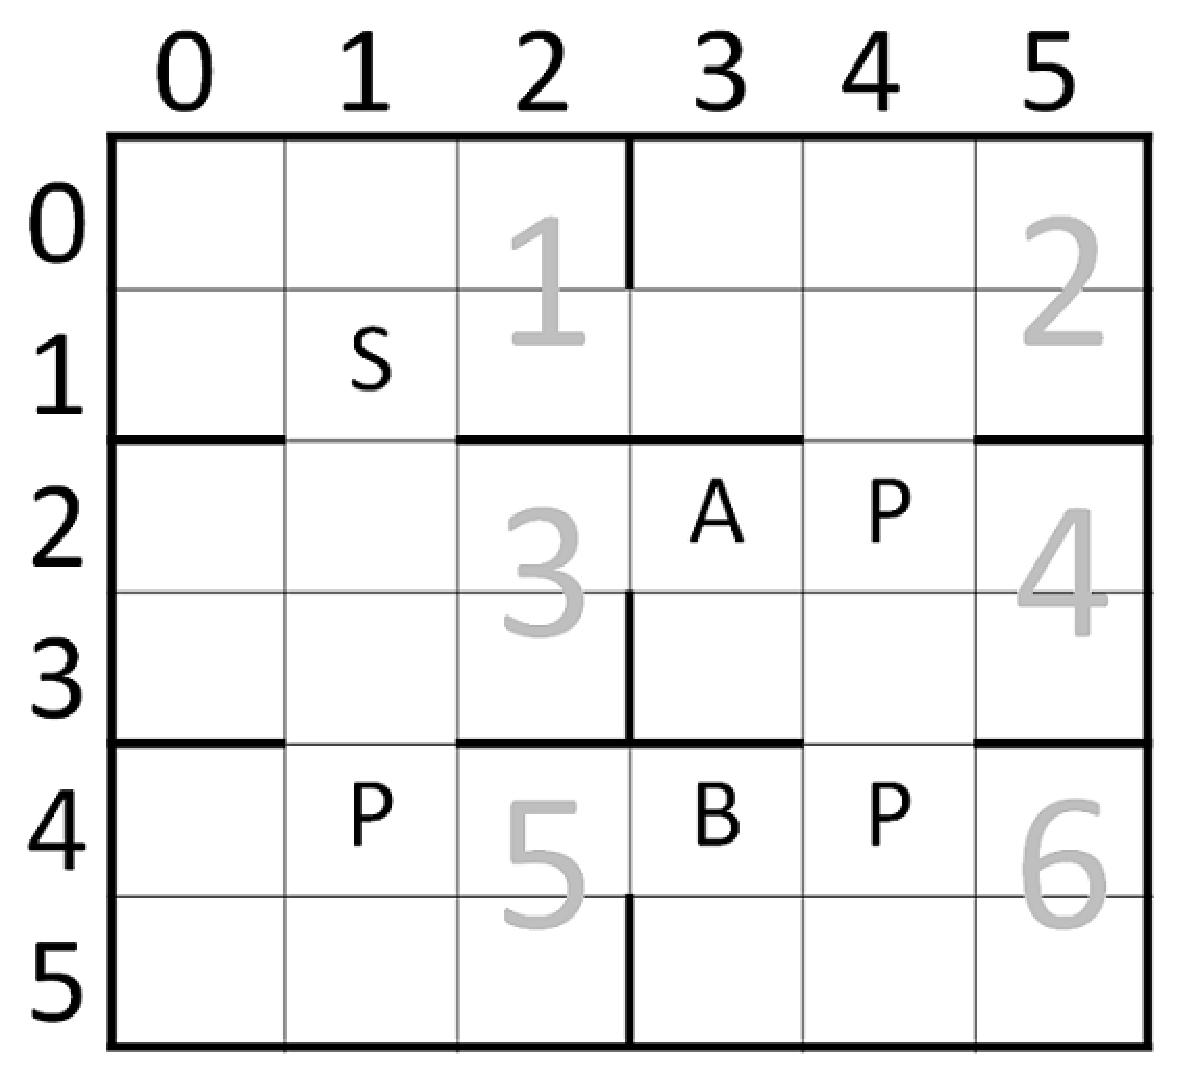
\includegraphics[width=2.5in] {BusSmall.eps}
    %\caption{(a)}
\end{minipage}
\begin{minipage}[b]{0.5\linewidth}
    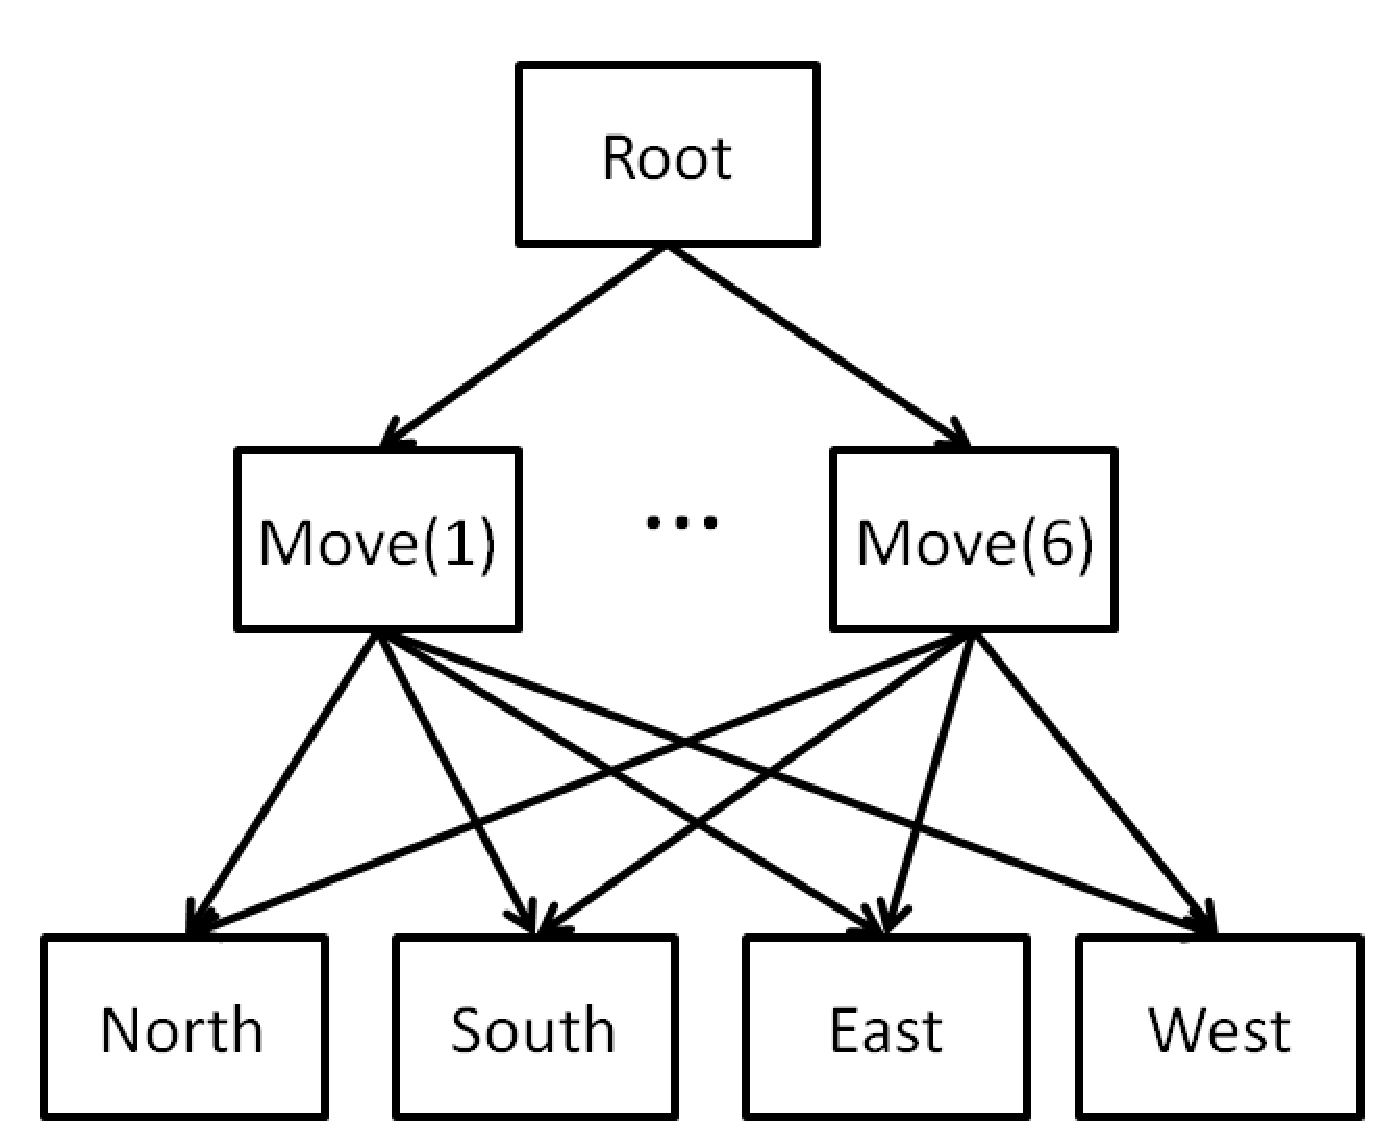
\includegraphics[width=2.5in] {BusHierarchy.eps}
\end{minipage}
\begin{minipage}[b]{0.5\linewidth} \centering (a) \end{minipage}
\begin{minipage}[b]{0.5\linewidth} \centering (b) \end{minipage}

%\end{center}
\caption{(a) The School Bus Domain (b) A task graph for the School Bus problem.}
\label{fig:bus}
\end{figure}

We test our approach in the school bus problem. School bus starts at school $S$. Its task 
is to pickup all of three passengers marked as $P$ and return to the school(Figure \ref{fig:bus}a).
The episode ends when it finishes the task. There are no reward for finishing the task.
The passengers can be picked up in any order. The bus picks up the passenger automatically when it moves into
the location of passenger.

The bus can move North, South, East, or West. There is a reward of -1 for each action.
There are two locations which may be under road construction. They are marked as 
$A$ and $B$. If the bus pass any construction site, it will get damaged with probability 1 and has probability
0.25 to break down for each step. There is a reward of -50 if the bus breaks down and the episode ends immediately. 

A state can be described by 8-tuple $(x, y, h, p_1, p_2, p_3, a, b)$, where $(x, y)$ is the location of 
bus, $h$ shows if the bus is damaged, $p_i$ indicates if the corresponding passenger has been picked up or not,
and $a$ and $b$ indicate the status of the construction sites.
%TODO: randomness in the game



%TODO: total leaf cover always exist
There are 4 primitive actions that move the bus one step North, South, East, or West. 
The world is divided by 6 areas. Composite action $Move(t)$ moves the bus to area $t$. 
$Move(t)$ can only be invoked if $t$ is the adjacent area.
%TODO: pesudo reward and terminates
Our hierarchy design specifies that

The task graph is shown in Figure \ref{fig:bus}(b). 
Since the six composite actions cover all primitive actions, they are a total leaf cover.
We used HORDQ in their corresponding subtasks to guarantee the convergence to the optimal
policy. $Root$ subtask adopted our approximated model-based method. The planning variables include 
the location of bus and the status of passengers. The environment variables are the 
damage status of bus and the status of road. 

Our model learns when the bus is damaged, it will receive a large penalty.  
Since the damage status is assumed static during the planning process, 
it fails to learn that the bus will get damaged if it passes through
location $A$ and $B$. Our model is certainly biased in this case, and
it cannot learn the optimal policy. One solution is to include the damage 
status as one of the planning variables. However, the objective of 
the experiment is to show that the optimal policy can be achieved
with the biased model if we combine it with HORDQ. 

Figure ??? shows the result with different pseudo rewards. 
With pseudo reward +60, the agent learned a suboptimal policy because
the pseudo reward is large enough to make $Move(t)$ subtask ignore 
the penalty of breakdown. As a result, The subtask followed 
the instruction of its parent strictly.

On other hand, if we do not impose any pseudo reward, 
the optimal policy can be learned, but the convergence rate is
slower than flat SARSA learning. Since the subtask has no
incentive to follow the instruction from the hierarchy, 
the learning process is similar to flat SARSA learning 
except it has six different Q-functions to learn (one for each subtask) instead of one.
Therefore it takes longer to learn the optimal policy. 

With appropriate pseudo reward, we can get a near-optimal policy
while the convergence rate is faster than flat SARSA learning.
Note that the pseudo reward of +5 is enough to make $Move(t)$ subtask follow 
the order of $Root$ in most of the times, but it is not large enough for $Move(t)$ to ignore
the breakdown penalty. When $Root$ wants to move the bus from area 
3 to area 4 and the road at location $A$ is under construction, $Move(4)$ subtask
will learn it is a bad decision with HORDQ.
Instead of moving to area 4, $Move(4)$ may move to area 1 or 5 to avoid
the breakdown penalty. In turn, $Root$ learns $Move(4)$ can not be done in 
such scenario, thus it will seek an alternate plan if the same scenario
is encountered.

In order to show the convergence 
The worst case of 

The result shows that we still need an approximately good model 
to enjoy the increase of convergence rate. However, 
it will converge to the optimal policy regardless of the quality of model.

On the contrary, the combination of MAXQ and a poor approximated model has
a performance similar to random policy.

%TODO: add random agent experiment
%TODO: if I set the pseudo reward to zero, will the whole stuff breaks down again?





%Place one line space before the table title, one line space after the table
%title, and one line space after the table. The table title must be lower caseggg
%Systems 7}, pp. 609-616. Cambridge, MA: MIT Press.

%[2] Bower, J.M. \& Beeman, D. (1995) {\it The Book of GENESIS: Exploring
%Realistic Neural Models with the GEneral NEural SImulation System.}
%New York: TELOS/Springer-Verlag.

%[3] Hasselmo, M.E., Schnell, E. \& Barkai, E. (1995) Dynamics of learning
%and recall at excitatory recurrent synapses and cholinergic modulation
%in rat hippocampal region CA3. {\it Journal of Neuroscience}
%{\bf 15}(7):5249-5262.
%}

{\small
\bibliographystyle{plain}
\bibliography{biblio}
}
\end{document}

\endinput
